\chapter{Geographic View}
\label{sec:geo_view}

The Geographic View allows a graphical representation of target reports from the DBContent. After creation, it displays a world map in the map widget on the left, and a configuration panel on the right hand side.

\subfile{geo_layout}

\subfile{geo_toolbar}

\subfile{geo_data_widget}

\subfile{geo_config_panel}

\section{Import of GeoTIFF Files}

External GeoTIFF files can be imported into Geographic View by dragging and dropping them into Geographic Views map view.

\begin{figure}[H]
  \center
    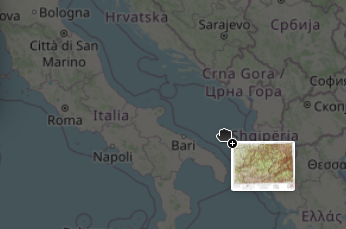
\includegraphics[width=12cm]{figures/geoview_import_geotiff.png}
  \caption{Import of a GeoTIFF file into Geographic View via drag and drop}
\end{figure}


This will open a dialog listing all added files with a supported GeoTIFF file extension.

\begin{figure}[H]
  \center
    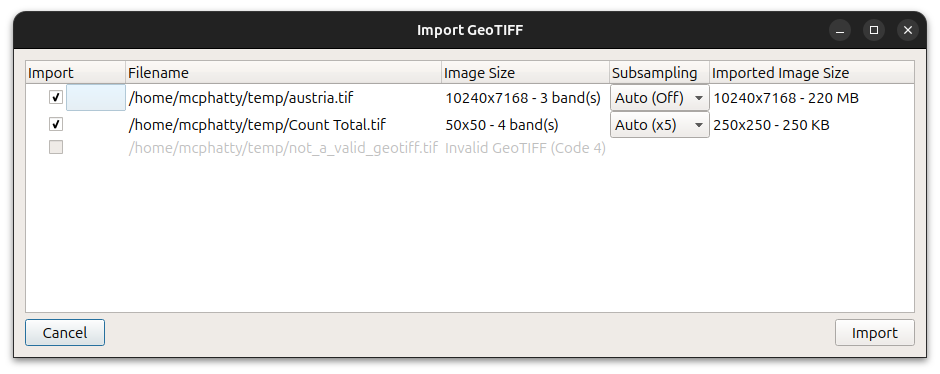
\includegraphics[width=12cm]{figures/geoview_import_geotiff_dialog.png}
  \caption{Import GeoTIFF dialog}
\end{figure}

The checkboxes in the 'Import' column can be used to again make a selection of which file to import.
The 'Information' column will either show information about the image size, or an error message in case 
the added file is not a valid GeoTIFF. \\

In the 'Subsampling' column the number of subsamples per image pixel can be chosen for each file.
Subsampling helps to avoid display artifacts at the cost of higher resolution and also memory consumption.
\textbf{Note} that each pixel will be subsampled in both x- and y-direction, resulting in e.g. 4 times 
the number of pixels for a subsampling of 2. In the column 'Imported Image Size' the resulting final image size and memory consumption 
is listed for each image. The 'Auto' mode tries to choose the maximum possible subsampling, while limiting
memory consumption to a reasonable extent. \\

Pressing the 'Import' button will start the import. \\

If the import succeeds the imported grid data will be listed in the 'Layer' tab under \textit{Annotations}$\rightarrow$\textit{Grids}. 
Interaction with these items is explaned in section \ref{sec:geo_annotation_ops}. \\

Imported GeoTIFF files will persist until COMPASS is closed. \\

\begin{figure}[H]
  \center
    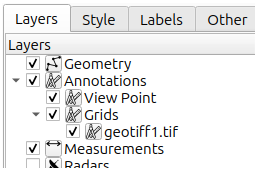
\includegraphics[width=6cm]{figures/geoview_import_geotiff_anno.png}
  \caption{Imported GeoTIFF files listed Geographic View's Layer tab}
\end{figure}
